\section{Trigonometrie}
\subsection{Winkelargumente}
\renewcommand{\arraystretch}{1.5}
\begin{tabular}{|c|c|c|c|c|c|c|c|c|c|c|c|c|c|c|c|c|c|c|c|c|}
	\hline \textbf{deg °} & $0$& $30$& $45$& $60$ &$90$&$120$& $135$&$150$&$180$ &$210$&$225$&$240$&$270$&$300$&$315$&$330$\\
	\hline \textbf{rad} & $0$& $\frac{\pi}{6}$&$\frac{\pi}{4}$&$\frac{\pi}{3}$&$\frac{\pi}{2}$&$\frac{2\pi}{3}$&$\frac{3\pi}{4}$&$\frac{5\pi}{6}$ &$\pi$&$\frac{7\pi}{6}$&$\frac{5\pi}{4}$&$\frac{4\pi}{3}$&$\frac{3\pi}{2}$&$\frac{5\pi}{3}$&$\frac{7\pi}{4}$&$\frac{11\pi}{6}$\\ 
	\hline \textbf{sin}&$0$&$\frac{1}{2}$&$\frac{\sqrt{2}}{2}$&$\frac{\sqrt{3}}{2}$&$1$&$\frac{\sqrt{3}}{2}$& $\frac{\sqrt{2}}{2}$&	$\frac{1}{2}$&$0$&$-\frac{1}{2}$ &$-\frac{\sqrt{2}}{2}$ &$-\frac{\sqrt{3}}{2}$ &$-1$&$-\frac{\sqrt{3}}{2}$ &$-\frac{\sqrt{2}}{2}$&$-\frac{1}{2}$\\
	\hline \textbf{cos}&$1$&$\frac{\sqrt{3}}{2}$ &$\frac{\sqrt{2}}{2}$&$\frac{1}{2}$ &$0$&$-\frac{1}{2}$&$-\frac{\sqrt{2}}{2}$&$-\frac{\sqrt{3}}{2}$&$-1$&$-\frac{\sqrt{3}}{2}$&$-\frac{\sqrt{2}}{2}$& $-\frac{1}{2}$&$0$&$\frac{1}{2}$&$\frac{\sqrt{2}}{2}$&$\frac{\sqrt{3}}{2}$\\
	\hline
\end{tabular}

\begin{multicols}{2}
	\subsection{Additionstheoreme}
	$\sin(a \pm b)=\sin(a) \cdot \cos(b) \pm \cos(a) \cdot \sin(b)$\\
	$\cos(a \pm b)=\cos(a) \cdot \cos(b) \mp \sin(a) \cdot \sin(b)$\\	
	$\tan(a \pm b)=\dfrac{\tan(a) \pm \tan(b)}{1 \mp \tan(a) \cdot \tan(b)}$
	
	\subsection{Doppel- und Halbwinkel}	
	$\sin(2a)=2\sin(a)\cos(a)$\\
	$\cos(2a)=\cos^2(a)-\sin^2(a)$\\
	$\cos^2 \left(\frac{a}{2}\right)=\frac{1+\cos(a)}{2} \qquad
	\sin^2 \left(\dfrac{a}{2}\right)=\frac{1-\cos(a)}{2}$

	\subsection{Produkte}
	$\sin(a)\sin(b)=\frac{1}{2}(\cos(a-b)-\cos(a+b))$\\
	$\cos(a)\cos(b)=\frac{1}{2}(\cos(a-b)+\cos(a+b))$\\
	$\sin(a)\cos(b)=\frac{1}{2}(\sin(a-b)+\sin(a+b))$\\	
	
	\subsection{Summe und Differenz}
	$\sin(a)+\sin(b)=2 \cdot \sin \left(\frac{a+b}{2}\right) \cdot
	\cos\left(\frac{a-b}{2}\right)$\\
	$\sin(a)-\sin(b)=2 \cdot \sin \left(\frac{a-b}{2}\right) \cdot
	\cos\left(\frac{a+b}{2}\right)$\\
	$\cos(a)+\cos(b)=2 \cdot \cos \left(\frac{a+b}{2}\right) \cdot
	\cos\left(\frac{a-b}{2}\right)$\\
	$\cos(a)-\cos(b)=-2 \cdot \sin \left(\frac{a+b}{2}\right) \cdot
	\sin\left(\frac{a-b}{2}\right)$\\
	$\tan(a) \pm \tan(b)=\dfrac{\sin(a \pm b)}{\cos(a)\cos(b)}$\\
	
	\subsection{Potenzen}
	$\sin^2(a)+\cos^2(a)=1$\\
	$\sin^2(a)-\cos^2(a)=1-2\sin^2(a)$\\
	$\sin^2(a)=\frac{1}{2}(1-\cos(2a))$\\
	$\cos^2(a)=\frac{1}{2}(1+\cos(2a))$\\
	$\sin^3(a)=\frac{1}{4}(3\sin(a)-\sin(3a))$\\
	$\cos^3(a)=\frac{1}{4}(3\cos(a)-\cos(3a))$\\
\end{multicols}

\subsection{Quadrantenbeziehungen}
\begin{tabbing}
	xxxxxxxxxxxxxxxxxxxxxxxxxxxxxxxxxx \= \kill
	$\sin(-a)=-\sin(a)$ \> $\cos(-a)=\cos(a)$\\
	$\sin(\pi - a)=\sin(a)$ \> $\cos(\pi - a)=-\cos(a)$\\
	$\sin(\pi + a)=-\sin(a)$ \> $\cos(\pi +a)=-\cos(a)$\\
	$\sin\left(\frac{\pi}{2}-a \right)=\sin\left(\frac{\pi}{2}+a \right)=\cos(a)$ \>
	$\cos\left(\frac{\pi}{2}-a \right)=-\cos\left(\frac{\pi}{2}+a \right)=\sin(a)$  
\end{tabbing}

\subsection{Plots}
\begin{multicols}{3}
	\subsubsection{Sinus-Funktion}
	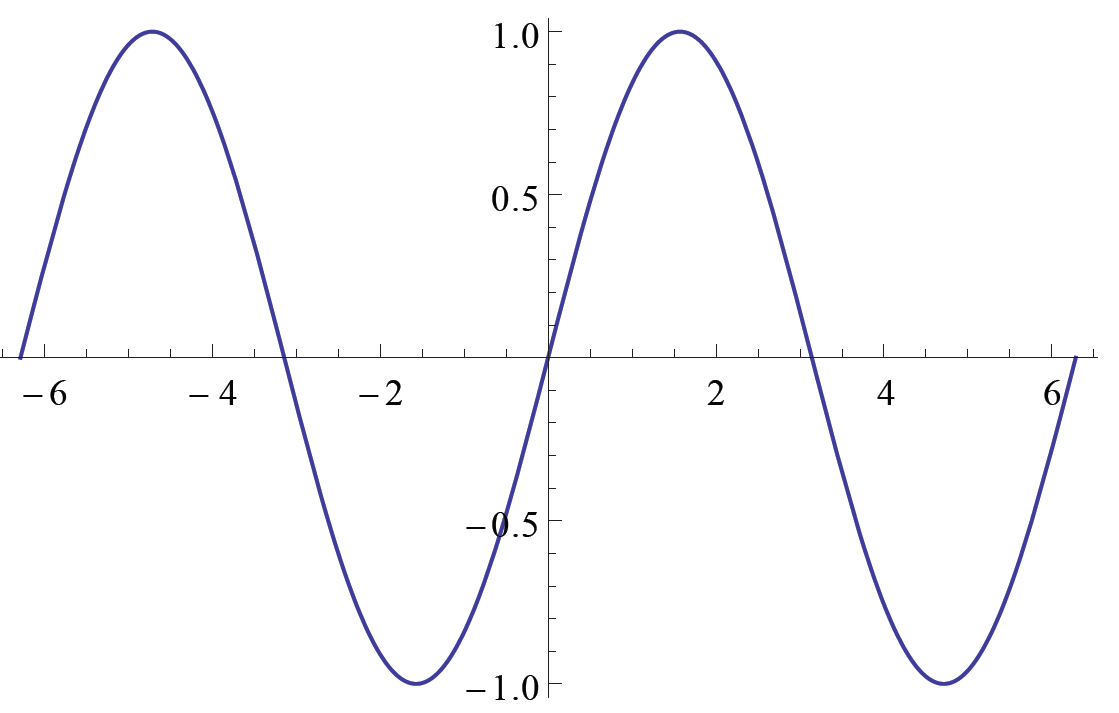
\includegraphics[width=5.5cm]{images/sin.png}
	\subsubsection{Cosinus-Funktion}
	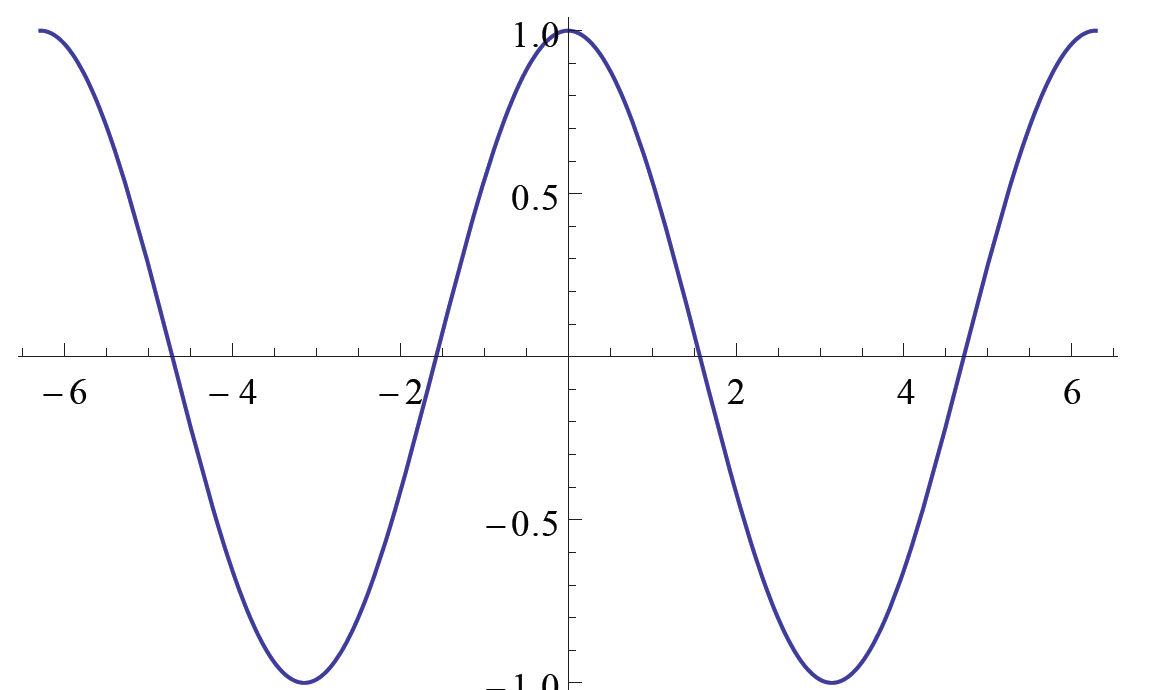
\includegraphics[width=5.5cm]{images/cos.png}
	\subsubsection{Tangens-Funktion}
	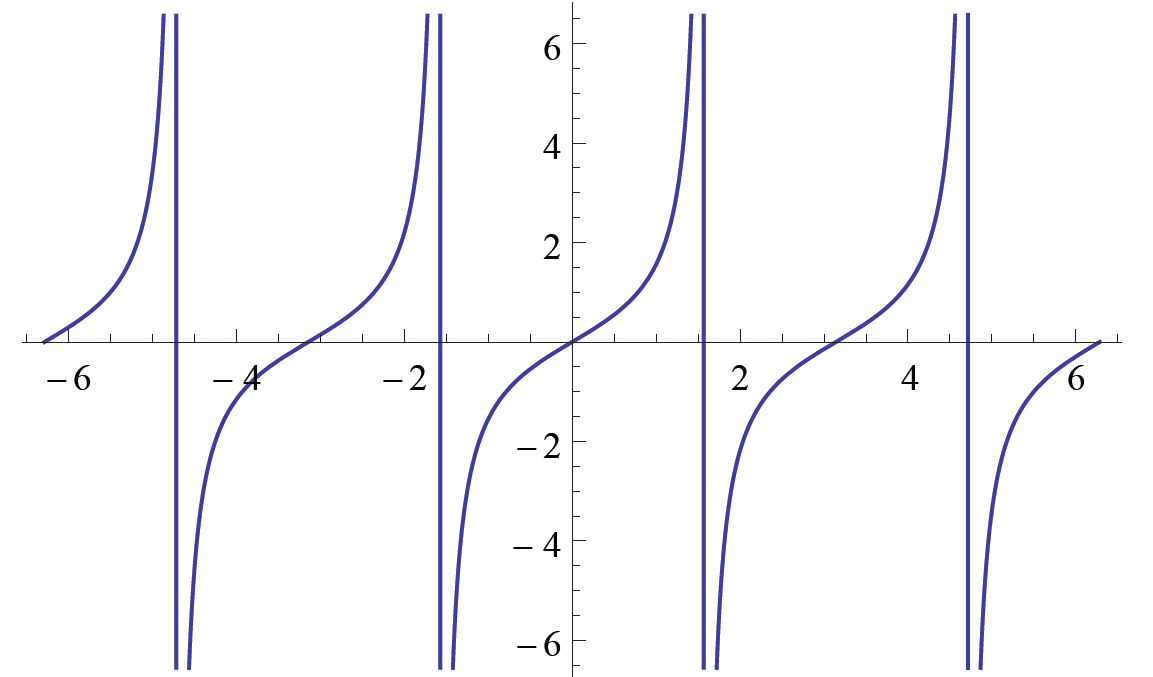
\includegraphics[width=5.5cm]{images/tan.png}
\end{multicols}